\subsubsection{1.2. Mô hình MGAT + FastKAN/MLP}
%===================================================================
\paragraph{1.2.1. Tầng trích xuất đặc trưng}
\indent\indent Đây là tầng đầu tiên tiếp nhận dữ liệu từ ba phương thức khác nhau. Kiến trúc của tầng này được minh họa tại \textbf{Hình \ref{fig:KTExtractFeaturesLayers}}, bao gồm ba nhánh xử lý độc lập:\vspace{-0.1cm}
\begin{itemize}[label={--}, itemsep=1pt]
    \item \textbf{Image Extractor:} Sử dụng backbone CNN đã được đóng băng tham số và BatchNorm để trích xuất đặc trưng hình ảnh. Đầu ra từ backbone được đưa qua một tầng Linear để chiếu về chiều không gian vector mong muốn (448 chiều).
    \item \textbf{Text Extractor:} Kết hợp vector embedding của từ (Word) và câu (Sentence).
    \item \textbf{Audio Extractor:} Xử lý đặc trưng MFCC kết hợp với các giá trị Delta và Delta-Delta.
\end{itemize}

\begin{figure}[H]
    \centering
    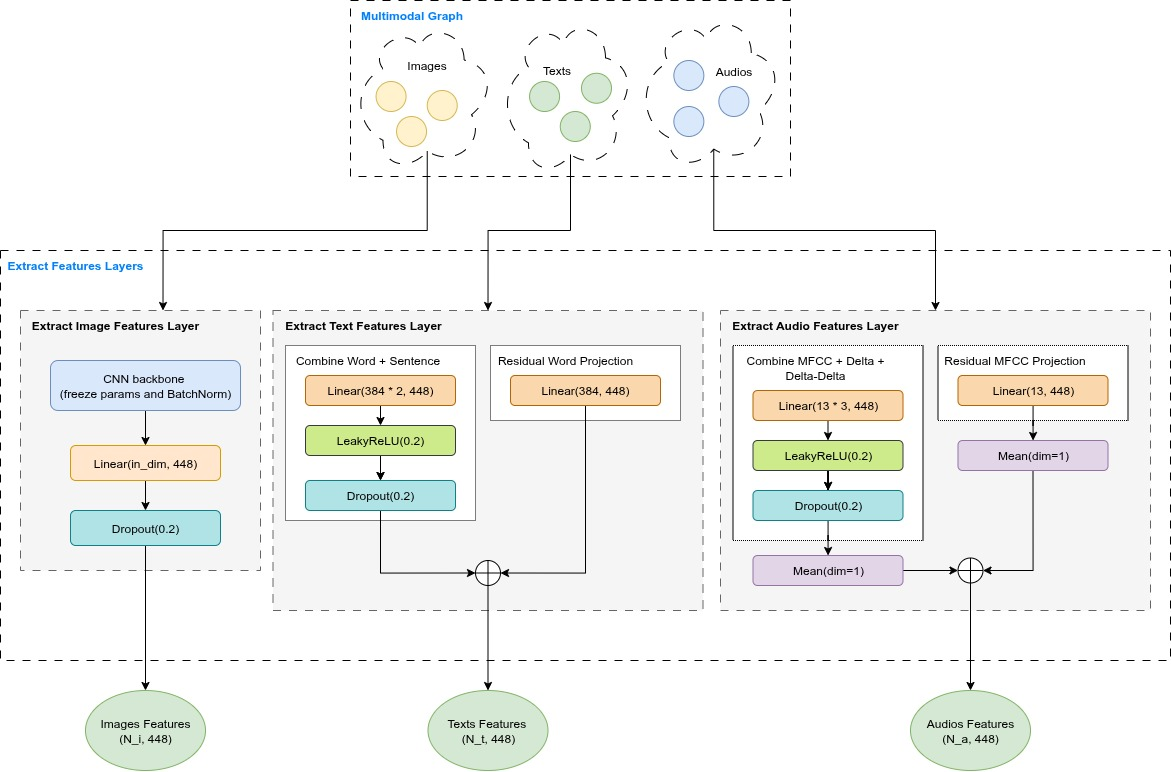
\includegraphics[width=\linewidth]{images/part-02/chap-02/sec-01/ExtractFeaturesLayers.jpg}
    \vspace{0.3cm}
    \caption{Kiến trúc chi tiết của Extract Features Layers}
    \label{fig:KTExtractFeaturesLayers}
\end{figure}

Đối với nhánh đặc trưng hình ảnh, do backbone đã cung cấp các vector đặc trưng giàu thông tin ngữ nghĩa, hệ thống chỉ áp dụng phép chiếu tuyến tính đơn giản. Ngược lại, đối với văn bản và âm thanh, hệ thống áp dụng cơ chế Residual Connection bằng cách cộng vector đặc trưng gốc (đã được chiếu về cùng chiều) vào đầu ra cuối cùng của nhánh. Kỹ thuật này giúp giải quyết vấn đề triệt tiêu đạo hàm khi huấn luyện mạng sâu, đồng thời bảo toàn thông tin gốc quan trọng trước các phép biến đổi phi tuyến có thể gây mất mát thông tin đặc trưng \cite{he2015deepresiduallearningimage}.
%===================================================================
\paragraph{1.2.2. Tầng chiếu không gian chung}
\indent\indent Mục tiêu của tầng này là đồng bộ hóa các vector đặc trưng từ ba phương thức khác nhau về cùng một không gian biểu diễn có số chiều cố định (512 chiều), với kiến trúc chi tiết tại \textbf{Hình \ref{fig:KTShareProjectionLayer}}.

\begin{figure}[H]
    \centering
    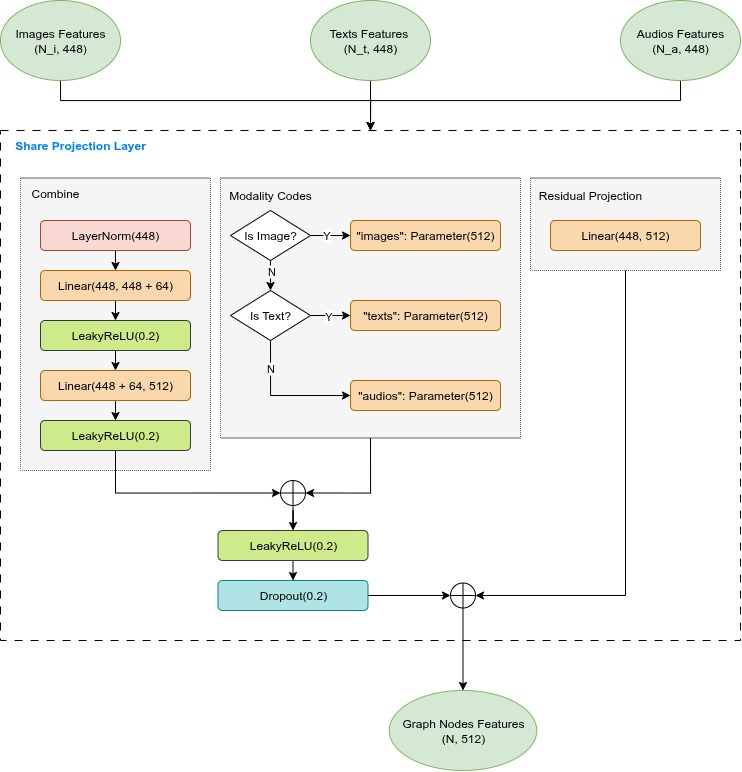
\includegraphics[width=0.8\linewidth]{images/part-02/chap-02/sec-01/ShareProjectionLayer.jpg}
    \vspace{0.3cm}
    \caption{Kiến trúc của Share Projection Layer}
    \label{fig:KTShareProjectionLayer}
\end{figure}

Để mô hình phân biệt được nguồn gốc của từng vector đặc trưng trong không gian chung, hệ thống sử dụng kỹ thuật \textit{Modality Embeddings} (hay Modality Codes). Mỗi phương thức được gán một vector tham số học được riêng biệt, cộng trực tiếp vào đặc trưng đầu ra nhằm ``đánh dấu'' vị trí của nó trong không gian vector chung. Kỹ thuật này được lấy cảm hứng từ cơ chế \textit{Token Type Embeddings} trong mô hình BERT, giúp mô hình nhận biết ngữ cảnh phương thức \cite{devlin2019bertpretrainingdeepbidirectional}. Đồng thời, cơ chế Residual Connection tiếp tục được áp dụng tại đây nhằm duy trì luồng thông tin xuyên suốt, tránh sự mất mát dữ liệu do các phép biến đổi không gian.
%===================================================================
\paragraph{1.2.3. Tầng học trọng số cạnh}
\indent\indent Tầng này đóng vai trò khởi tạo cấu trúc đồ thị bằng cách xác định độ mạnh yếu của các liên kết giữa các đỉnh, như minh họa tại \textbf{Hình \ref{fig:KTEdgeWeightsLayer}}.

\begin{figure}[H]
    \centering
    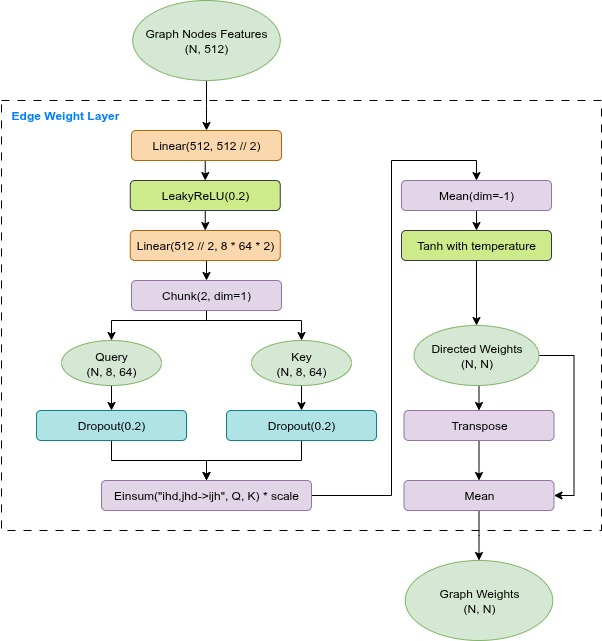
\includegraphics[width=0.8\linewidth]{images/part-02/chap-02/sec-01/EdgeWeightsLayer.jpg}
    \vspace{0.3cm}
    \caption{Kiến trúc của Edge Weights Layer sử dụng cơ chế Attention}
    \label{fig:KTEdgeWeightsLayer}
\end{figure}

Mạng học trọng số được thiết kế dựa trên cơ chế \textit{Self-Attention} với tích vô hướng $Q \cdot K^T$ để nắm bắt tương quan ngữ nghĩa \cite{vaswani2023attentionneed}. Đặc biệt, đầu ra sử dụng hàm kích hoạt \texttt{Tanh} để giới hạn giá trị trong khoảng $[-1, 1]$. Việc cho phép trọng số âm tại bước này đóng vai trò như một cơ chế "lọc mềm" (soft thresholding): các giá trị âm sẽ được quy về 0 bởi hàm \texttt{Clamp(min=0)} ở các tầng tiếp theo, giúp mô hình chủ động học cách ngắt bỏ các kết nối nhiễu hoặc không liên quan thay vì buộc phải duy trì tất cả các cạnh với trọng số dương nhỏ. Bên cạnh đó, để đảm bảo tính vô hướng của đồ thị, tôi thêm vào phép tính trung bình cộng giữa ma trận trọng số với ma trận chuyển vị của chính nó, điều này đảm bảo rằng trọng số kết nối từ đỉnh A đến đỉnh B và ngược lại là như nhau.
%===================================================================
\paragraph{1.2.4. Tầng GAT}
\indent\indent Đây là thành phần cốt lõi thực hiện quá trình truyền tin (Message Passing) để cập nhật đặc trưng đỉnh, với kiến trúc được minh hoạ như \textbf{Hình \ref{fig:KTGATLayers}}.

\begin{figure}[H]
    \centering
    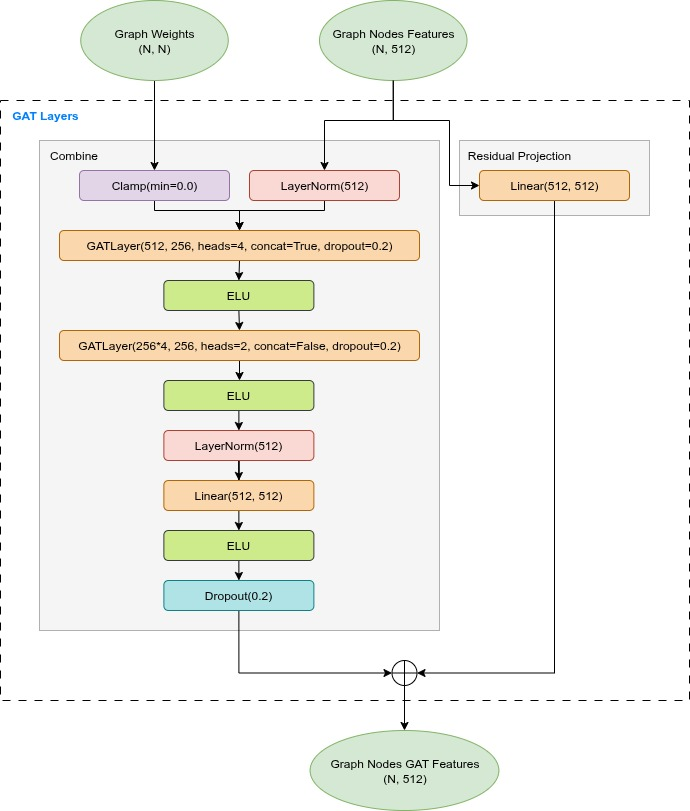
\includegraphics[width=0.8\linewidth]{images/part-02/chap-02/sec-01/GATLayers.jpg}
    \vspace{0.3cm}
    \caption{Kiến trúc của GAT Layers với cơ chế Weighted Message Passing}
    \label{fig:KTGATLayers}
\end{figure}

Hệ thống áp dụng biến thể \textbf{Weighted GAT} kết hợp với \textit{Dynamic Attention}. Khác với GAT truyền thống chỉ dựa vào đặc trưng nút và ma trận kề để tính hệ số attention, thì mô hình của tôi tích hợp trực tiếp trọng số cạnh học được ($GW_{ij}$) vào quá trình tính toán:
\[
    \alpha_{ij} = \text{softmax}(\text{LeakyReLU}(\vec{a}^T [W\vec{h}_i \| W\vec{h}_j]) \cdot {GW}_{ij})
\]
\indent Trong đó $GW_{ij}$ là ma trận trọng số cạnh của đồ thị từ tầng trước đã qua hàm \texttt{Clamp(min=0.0)} để loại bỏ giá trị âm. Cơ chế này giúp khắc phục hạn chế "Static Attention", cho phép mô hình kiểm soát dòng chảy thông tin linh hoạt hơn: các cạnh có trọng số lớn sẽ khuếch đại tín hiệu, ngược lại các cạnh yếu sẽ bị chặn lại. Hàm kích hoạt phi tuyến ELU (Exponential Linear Unit) được sử dụng sau mỗi lớp GAT nhằm hỗ trợ việc học các biểu diễn mạnh mẽ hơn và tăng tốc độ hội tụ so với ReLU tiêu chuẩn \cite{clevert2016fastaccuratedeepnetwork}.\vspace{0.3cm}

Ngoài ra, tại tầng này tôi sử dụng thêm kỹ thuật \textit{Pre-LayerNorm} (chuẩn hóa trước khi đưa vào layer) để ổn định gradient khi huấn luyện mô hình sâu, tránh hiện tượng bùng nổ hoặc triệt tiêu gradient thường gặp trong các mạng GNN nhiều lớp \cite{xiong2020layernormalizationtransformerarchitecture}. Tương tự các tầng trước, cơ chế Residual Connection vẫn được duy trì để bảo toàn thông tin gốc qua các phép biến đổi phức tạp.
%===================================================================
\paragraph{1.2.5. Bộ phân lớp}
\indent\indent Tầng cuối cùng thực hiện ánh xạ từ không gian đặc trưng đồ thị sang không gian nhãn xác suất, sử dụng tùy chọn FastKAN hoặc MLP như minh họa tại \textbf{Hình \ref{fig:KTClassifier}}.

\begin{figure}[H]
    \centering
    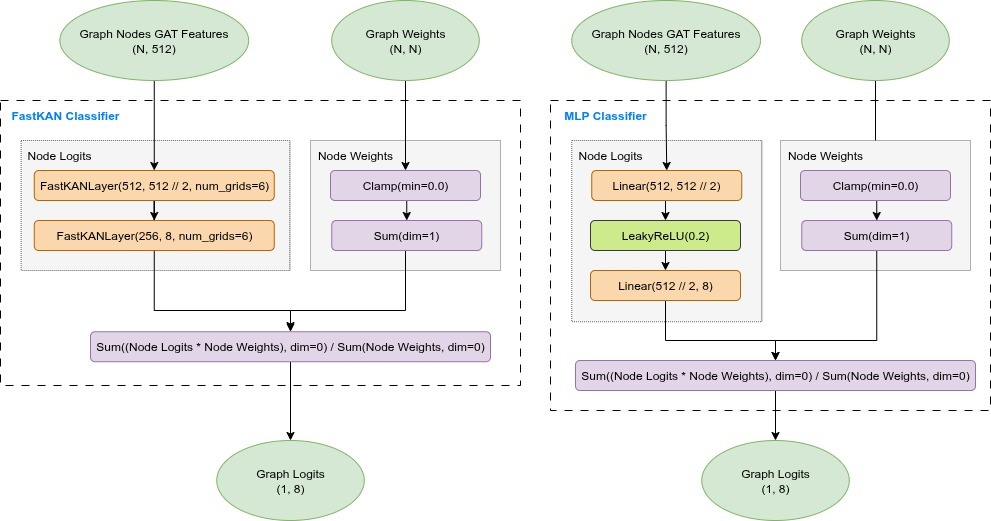
\includegraphics[width=\linewidth]{images/part-02/chap-02/sec-01/Classifier.jpg}
    \vspace{0.3cm}
    \caption{Kiến trúc bộ phân lớp bằng FastKAN và MLP}
    \label{fig:KTClassifier}
\end{figure}

Thay vì sử dụng kỹ thuật \textit{Global Mean Pooling} thông thường (coi vai trò các đỉnh là như nhau), tôi áp dụng cơ chế \textit{Weighted Voting (Bầu chọn có trọng số)}. Kết quả dự đoán cuối cùng là trung bình có trọng số của các dự đoán từ từng đỉnh ($logits_i$), dựa trên tổng trọng số kết nối dương ($d_i = \sum_j w_{ij}$) của đỉnh đó:
\[
    y_{pred} = \frac{\sum_i (logits_i \cdot d_i)}{\sum_i d_i + \epsilon}
\]
\indent Trong đó $\epsilon$ là hằng số nhỏ để tránh lỗi chia cho 0. Cơ chế này phù hợp với lý thuyết về \textit{Graph Readout Operations}, khẳng định rằng việc tổng hợp thông tin dựa trên cấu trúc giúp mô hình ưu tiên các đỉnh trung tâm giàu thông tin và giảm thiểu tác động của các đỉnh nhiễu ngoại lai \cite{xu2019powerfulgraphneuralnetworks}.